

\chapter{Combinational Loops}

\section{Introduction}

In this chapter we deal with \textit{loop} concept from hardware perspective, and see how to implement it using \verb|HLS|.\\

\todo{Intro combinational loop} \uti{Intro combinational loop:}

\begin{itemize}

\item \textit{To rewrite it later after finishing the chapter}

\end{itemize}

\newpage
\section{Definition}

$\mathrm{1}^\mathrm{st}$ let's take an example of \verb|for| loop statement, and see the scenrios in a software perspective, then move to hardware perspective. The example of software perspective is shown in \autoref{fig:comb_loop:loop_soft}.


\begin{figure}[h]
\centering
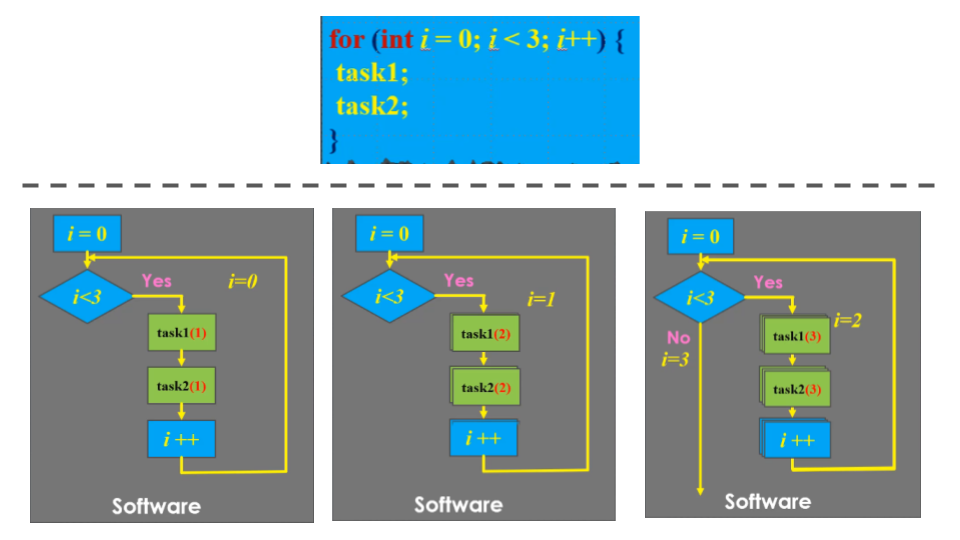
\includegraphics[scale=0.40,frame]{Figures/comb_loop/loop_soft}
\caption{For loop in a software execution}
\label{fig:comb_loop:loop_soft}
\end{figure}

\begin{itemize}

\item Notice that in each iteration, each \verb|task1| \verb|task2| has 1 instance invoked

	\begin{itemize}
	\item In other words, have 1 instance of \verb|taks1| and \verb|task2| used in all executions (iterations)
	\end{itemize}

\end{itemize}

Now unlike software concept, in hardware we have different instances (more like circuit modules) for each task in each iteration. In the \verb|for| loop example of \autoref{fig:comb_loop:loop_soft}, we have 3 iterations and 2 \verb|taskx| (\verb|1| and \verb|2|), so we obtain 6 instnaces in total, 3 for each \verb|task|.

Now concerning the flow of the loop, it is related to the  \tbi{dependency among data and iterations} between the tasks. 

\newpage
All different cases are shown in  \autoref{fig:comb_loop:loop_hardware}.

\begin{figure}[h]
\centering
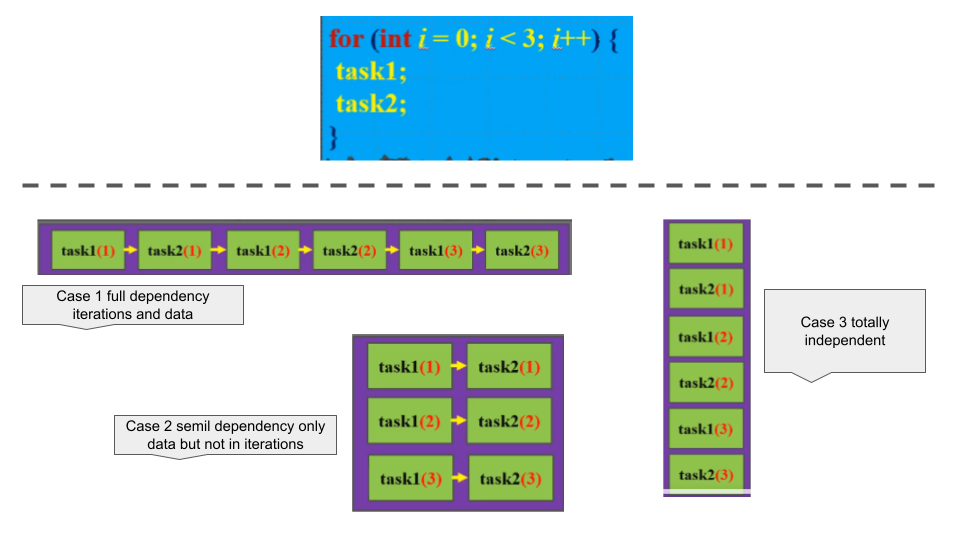
\includegraphics[scale=0.45,frame]{Figures/comb_loop/loop_hardware}
\caption{For loop in a hardware execution}
\label{fig:comb_loop:loop_hardware}
\end{figure}

\begin{itemize}

\item In case 1, because of full depdency, \verb|task2| need to wait for \verb|task1| (the data part), and in the next iterations also we need results, so \verb|task1(2)| need for both \verb|task1(1)| and \verb|task2(1)| to finish

	\begin{itemize}
	\item Full dependcy result in a sequential execution of the \verb|for| loop
	\end{itemize}

\item Case2 we only have dependncy among data, but not in iterations. This means \verb|task1(x)| in all iterations can run in parallel

\item Case 3 all the modules or instances are independent, hence all modules run in parallel.

\end{itemize}

\newpage
\subsection{Quiz}

\underline{Quiz 1:} Draw an execution graph for a  combinantional circuit that perform the \verb|for| loop shown in 
\autoref{fig:comb_loop:quiz_1_loop}.

\begin{figure}[h]
\centering
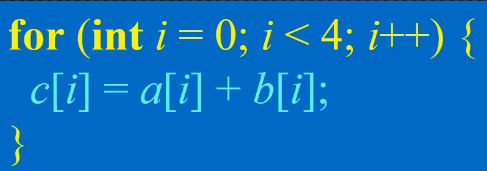
\includegraphics[scale=0.45,frame]{Figures/comb_loop/quiz_1_loop}
\caption{Quiz 1 for loop}
\label{fig:comb_loop:quiz_1_loop}
\end{figure}

\underline{Solution Quiz 1:} 
The data dependency plays a crucial role in the combinational circuit execution model. For this purpose, a graph can show the dependency relation between expressions. According to the \verb|for| loop body, the loop has three iterations that
are independent if arrays \verb|a|,\verb|b| and \verb|c| are stored in different memory areas.


Each iteration can be shown by a single graph node as shown in \autoref{fig:comb_loop:quiz_1_loop_graph}.


\begin{figure}[h]
\centering
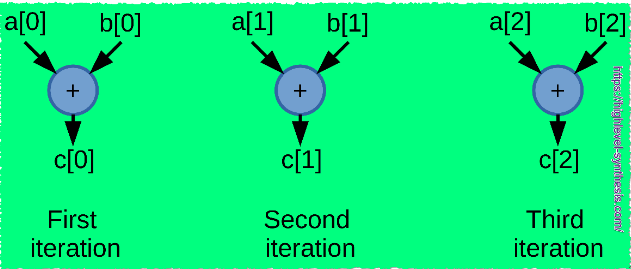
\includegraphics[scale=0.45,frame]{Figures/comb_loop/quiz_1_loop_graph}
\caption{Quiz 1 for loop graph}
\label{fig:comb_loop:quiz_1_loop_graph}
\end{figure}

As these iterations are independent, all of them can be executed in parallel that can be shown \autoref{fig:comb_loop:quiz_1_loop_execution}.

\begin{figure}[h]
\centering
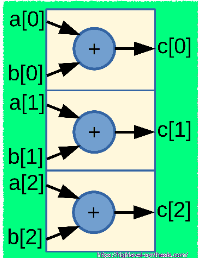
\includegraphics[scale=0.45,frame]{Figures/comb_loop/quiz_1_loop_execution}
\caption{Quiz 1 for loop execution}
\label{fig:comb_loop:quiz_1_loop_execution}
\end{figure}

\newpage
\underline{Quiz 2:} same as quiz 1, but the \verb|for| loop shown in \autoref{fig:comb_loop:quiz_2_loop}.

\begin{figure}[h]
\centering
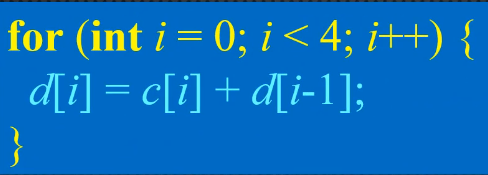
\includegraphics[scale=0.45,frame]{Figures/comb_loop/quiz_2_loop}
\caption{Quiz 2 for loop}
\label{fig:comb_loop:quiz_2_loop}
\end{figure}

\underline{Solution Quiz 2:}  As can be seen, each iteration of this for loop uses a data (denoted by $d[i-1]$) generated by its predecessor. Therefore, \tbi{there is a data dependency between two consecutive loop iterations in this code}.
Each addition in iteration can be seen by a graph node as shown in \autoref{fig:comb_loop:quiz_2_loop_graph}.

\begin{figure}[h]
\centering
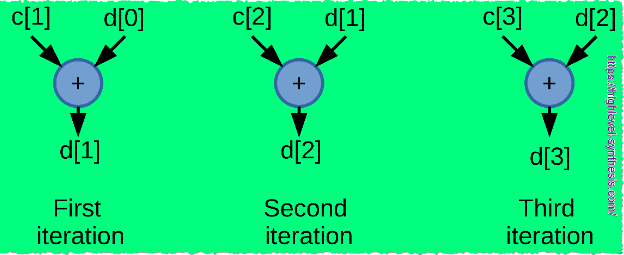
\includegraphics[scale=0.45,frame]{Figures/comb_loop/quiz_2_loop_graph}
\caption{Quiz 2 for loop graph}
\label{fig:comb_loop:quiz_2_loop_graph}
\end{figure}


These graph nodes should be executed one after another because of the data dependency between them. The dataflow graph in \autoref{fig:comb_loop:quiz_2_loop_execution} shows the hardware execution model of the \verb|for| loop.

\begin{figure}[h]
\centering
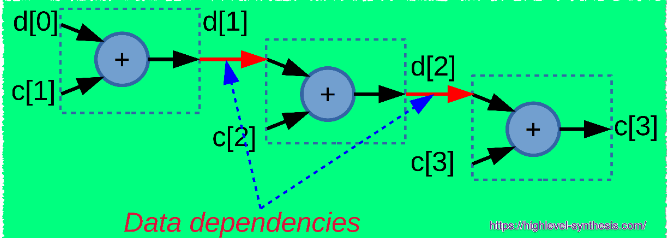
\includegraphics[scale=0.45,frame]{Figures/comb_loop/quiz_2_loop_execution}
\caption{Quiz 2 for loop execution}
\label{fig:comb_loop:quiz_2_loop_execution}
\end{figure}

\newpage
\section{Loop Unroll}

After presenting the concept of loop, let's see some actual code with some examples. We take $N$ bit binary adder shown in \autoref{fig:comb_loop:N_bit_binary_adder} (see \ref{sub:N_bit_binary_adder} for details). 


\begin{figure}[h]
\centering
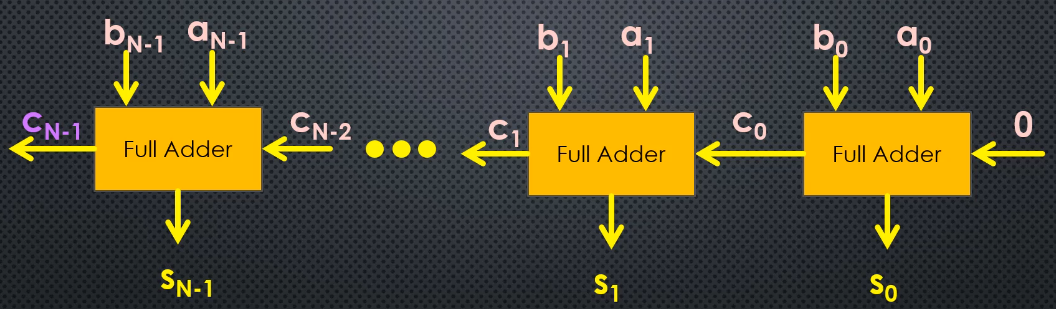
\includegraphics[scale=0.45,frame]{Figures/comb_loop/N_bit_binary_adder}
\caption{$N$ bit binary adder}
\label{fig:comb_loop:N_bit_binary_adder}
\end{figure}

The $N$ bit binary adder can be impelemted using \verb|for| loop as shown in \autoref{fig:comb_loop:loop_N_bit_adder}.

\begin{figure}[h]
\centering
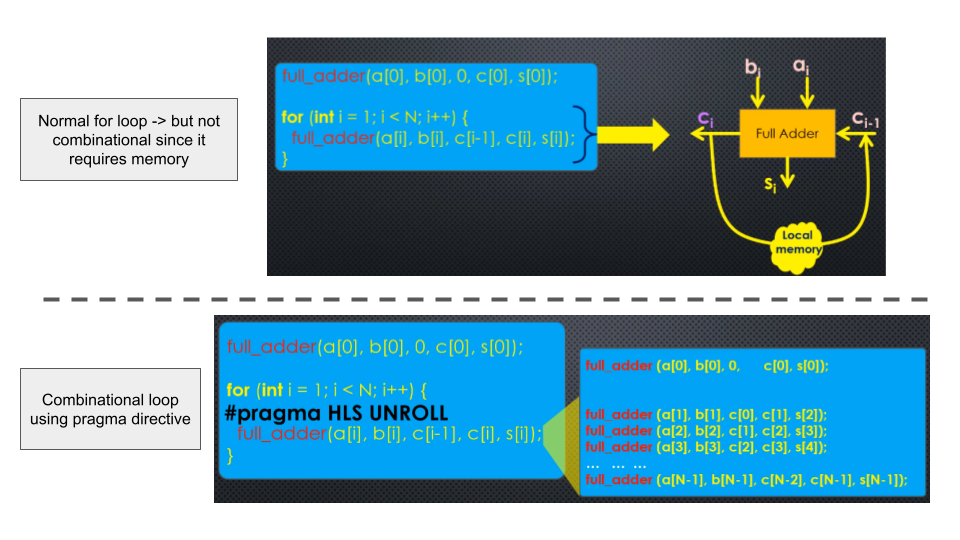
\includegraphics[scale=0.45,frame]{Figures/comb_loop/loop_N_bit_adder}
\caption{full-adder() function using for loop}
\label{fig:comb_loop:loop_N_bit_adder}
\end{figure}

\begin{itemize}

\item In the $\mathrm{1}^\mathrm{st}$ implementation, since we need the carry bit from the previous block, we need some kind of memory to track and save the result, resulting in a sequential circuit

\item To obtain a combinational circuit, we use the \verb|pragma unroll|, tell the \verb|for| loop to unroll the function \verb|full_adder()| and call it $N$ times, and no need for storage element

\end{itemize}

\subsection{Loop unroll condition}

Not every \verb|for| loop can be unrolled as shown in the $\mathrm{2}^\mathrm{nd}$ implementation in \autoref{fig:comb_loop:loop_N_bit_adder}. In order for the \verb|HLS| tool unroll a \verb|for| loop, the number of iteration need to be:

\begin{itemize}

\item known at compile time

\item in other words the number of iteration need to be bounded

\end{itemize}

\autoref{fig:comb_loop:loop_unroll_condition} shows some scenarios where a \verb|for| loop can be unrolled

\begin{figure}[h]
\centering
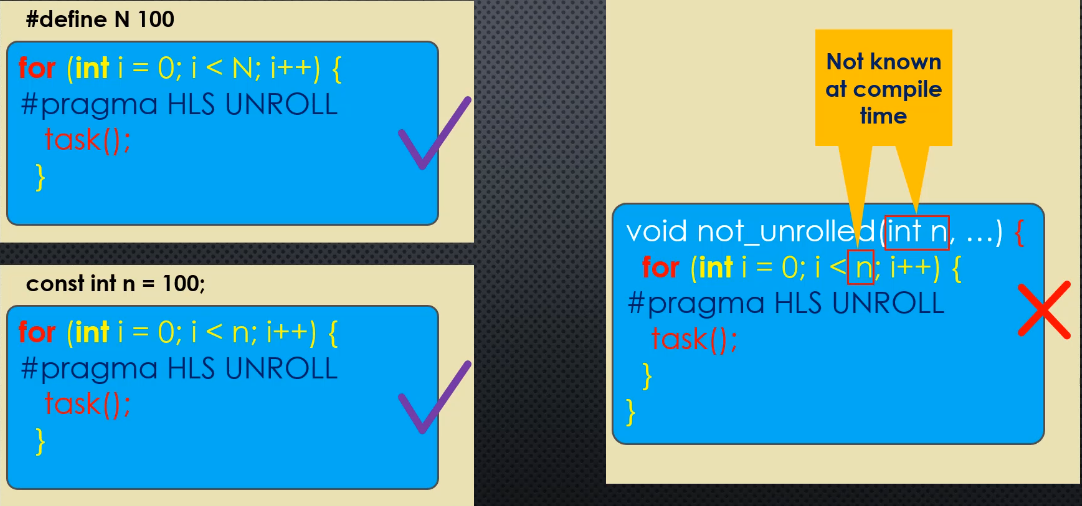
\includegraphics[scale=0.45,frame]{Figures/comb_loop/loop_unroll_condition}
\caption{Loop unroll condition}
\label{fig:comb_loop:loop_unroll_condition}
\end{figure}


\begin{itemize}

\item $\mathrm{1}^\mathrm{st}$ case \verb|N| is defined using a macro

\item $\mathrm{2}^\mathrm{nd}$ case \verb|n| is a variable but of type \verb|const|, so it can be unrolled

\item $\mathrm{3}^\mathrm{rd}$ case \verb|n| is a variable so it can be unrolled to combinational circuit

	\begin{itemize}
	\item \verb|HLS| tool will give a warning and sythethise the code into a sequential circuit
	\end{itemize}

\end{itemize}

\newpage
\subsection{Loop unroll resources}

When unrolling a \verb|for| loop, we need to be sure that the target FPGA has enough resources in order to implement the hardware needed for the \verb|for| loop.

That is because unrolling a \verb|for| loop, as done in \autoref{fig:comb_loop:loop_N_bit_adder}, result in different hardware instances.\\


\autoref{fig:comb_loop:loop_unroll_resources} shows an example of FPGA resources in terms of LUT.

\begin{figure}[h]
\centering
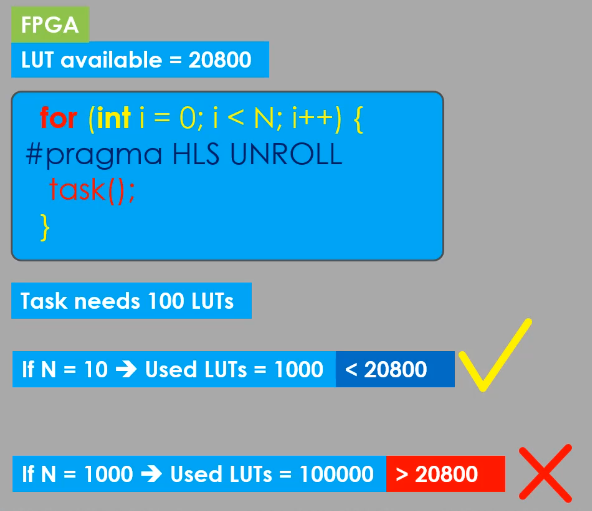
\includegraphics[scale=0.45,frame]{Figures/comb_loop/loop_unroll_resources}
\caption{Loop unroll resources}
\label{fig:comb_loop:loop_unroll_resources}
\end{figure}

\begin{itemize}

\item The \verb|task()| itself needs 100 LUT to be executed

\item So all depends on \verb|N|

	\begin{itemize}
	\item for \verb|N = 10|, we have enough resources
	
	\item for \verb|N = 100|,  the target FPGA lack of resources
	\end{itemize}

\end{itemize}

If the FPGA lack of resources, the synthesis tool (\verb|Vivado| in our case) complains and send some messages that it can't generate the bitstream file to program the FPGA.

\newpage
\subsection{Quiz}

\underline{Given:} which code in \autoref{fig:comb_loop:quiz_for_loop_combinational} can be synthesised into a combinational circuit ?


\begin{figure}[h]
\centering
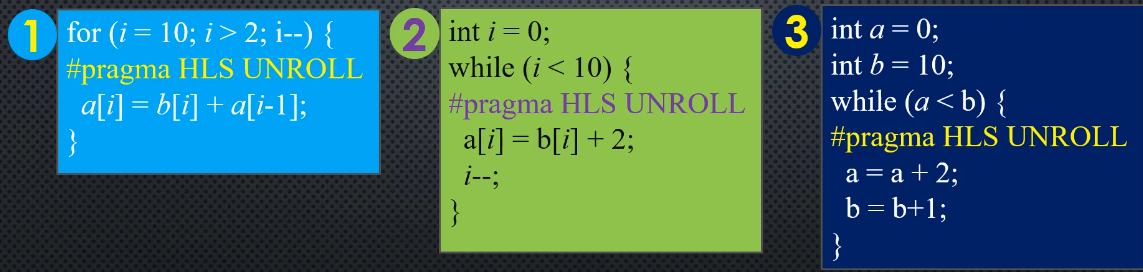
\includegraphics[scale=0.40,frame]{Figures/comb_loop/quiz_for_loop_combinational}
\caption{Quiz for loop}
\label{fig:comb_loop:quiz_for_loop_combinational}
\end{figure}

\underline{Solution:}

\begin{itemize}


\item The $\mathrm{1}^\mathrm{st}$ code can be synthesised into a combinational circuit as it has a static \verb|for| loop bound that can be determined at compile time 

\item The $\mathrm{2}^\mathrm{nd}$ code can also be synthesised into a combinational circuit as it has a static \verb|while| loop bound that can be determined at compile time

\item The $\mathrm{3}^\mathrm{rd}$ code cannot be synthesised into a combinational circuit as the loop bound determined as run-time based on the value assigned to a and b variables in each iteration.

\end{itemize}


\newpage
\section{Parity Bit}
\label{sec:parity_bit}

Now in this section we take a practical example to apply the loop mechanism seen so far in this chapter.\\

The parity bit is a technique to \tbi{detect a single bit error in binary data}. The binary bit stored in memory can undergoes some error during processing or transmission due to many phenomena (terrestrial radiations, magnetic fields,$\cdots$). The pheneomenon of error is so critical in many indsutries (nuclear, satellite,$\cdots$).\\


Single Event Upset (also known as soft-error) is one of the famous models representing this type of error. This model assumes that one of the binary bits changes its state from 0 $\rightarrow$ 1 or from 1 $\rightarrow$ 0 (as can be seen in \autoref{fig:comb_loop:parity_bit_intro}).

As an example, a Single Event Upset in the flight computers of Airbus A330 on 7 October 2008 is suspected to result in an aircraft upset that nearly ended in its crashing after the computers underwent several malfunctions.
  
\begin{figure}[h]
\centering
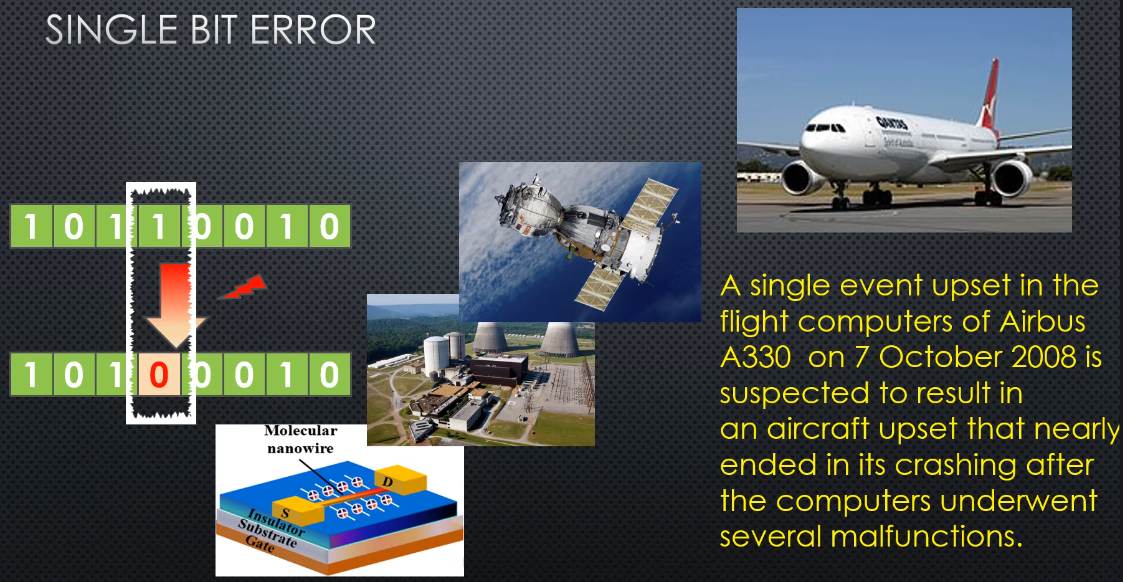
\includegraphics[scale=0.40,frame]{Figures/comb_loop/parity_bit_intro}
\caption{Parity bit and single event upset}
\label{fig:comb_loop:parity_bit_intro}
\end{figure}
 
\newpage
\subsection{Defintion of parity bit}

Now let's move to the defintion of this parity bit technique.

A parit bit is a one bit signature that is attached to the original $n$ bit data. The attachement can be doe via saving, or via transmission, and it is done by the parity generator.


\begin{figure}[h]
\centering
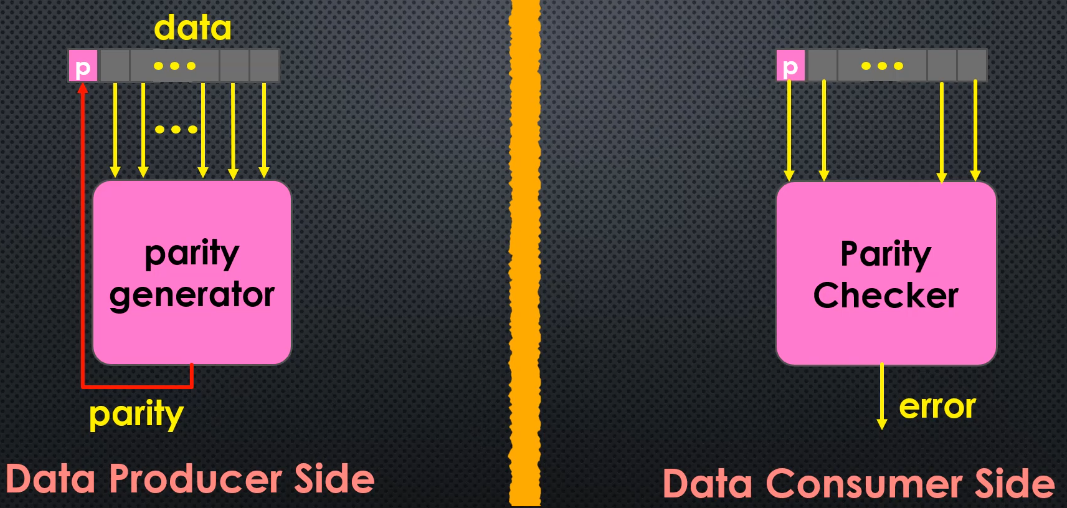
\includegraphics[scale=0.40,frame]{Figures/comb_loop/parity_bit_definition}
\caption{Parity bit definition}
\label{fig:comb_loop:parity_bit_definition}
\end{figure}

Then at the receiver side, the parity checker can check if we have some error in the data using this parity bit.

\newpage
\subsection{Parity types}

The parity is classified into 2 types: odd and even.

The general rule for odd or even is that the number of 1 in the data + parity bit should be even or odd. An example is shown in \autoref{fig:comb_loop:parity_types} to illustrate the concept.

\begin{figure}[h]
\centering
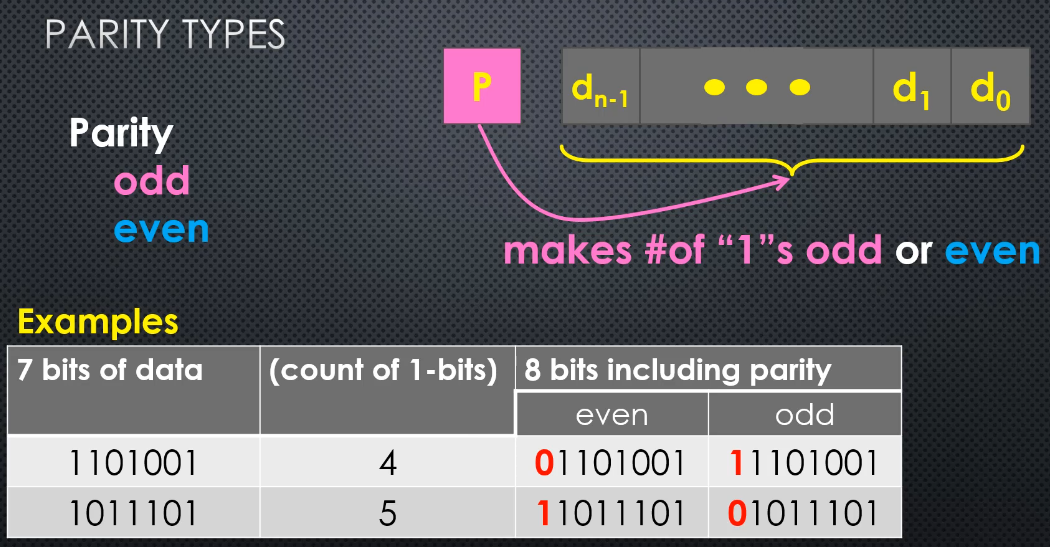
\includegraphics[scale=0.40,frame]{Figures/comb_loop/parity_types}
\caption{Parity types}
\label{fig:comb_loop:parity_types}
\end{figure}

\begin{itemize}

\item $\mathrm{1}^\mathrm{st}$ example where number of 1 $=$ 4

	\begin{itemize}
	\item If we want even parity, $\rightarrow$ parity bit should be 0 because 
	
	$ 4 \, (\,\text{in data}\,) \, + 0 \, = \, 4 \, (\,\text{even}\,)$
	
	\item If we want odd parity $\rightarrow$ parity bit should be 1 because 
	
	$ 4 \, (\,\text{in data}\,) \, + 1 \, = \, 5 \, (\,\text{odd} \,)$
	\end{itemize}

\item $\mathrm{2}^\mathrm{nd}$ example, number of 1 $=$ 5

	\begin{itemize}
	\item If we want even parity, the $\mathrm{8}^\mathrm{th}$ parity bit should be 1 because $5 \, + \ , 1 \, = \, 6 \, (\,\text{even}\,)$
	
	\item Same if we want for odd parity, he $\mathrm{8}^\mathrm{th}$ parity bit should be 0 because because 
	
	$5 \, + \ , 1 \, = \, 6 \, (\,\text{odd} \,)$

	\end{itemize}


\end{itemize}

\newpage
\subsection{Quiz}

The data in \autoref{fig:comb_loop:quiz_parity_bit} contain their parity bit , which one is erroneous ?

\begin{figure}[h]
\centering
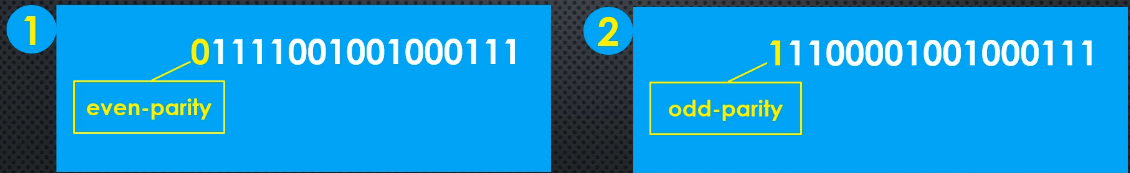
\includegraphics[scale=0.40,frame]{Figures/comb_loop/quiz_parity_bit}
\caption{Quiz parity bit}
\label{fig:comb_loop:quiz_parity_bit}
\end{figure}

\underline{Solution:}

\begin{itemize}

\item $\mathrm{1}^\mathrm{st}$ case: the data is erroneous as the number of ones in the data is 9, so then even parity should be 1, but it is 0

\item $\mathrm{2}^\mathrm{nd}$ case: this one also has an error as the number of ones is 7, so the odd-parity bit should be 0 but it is 1.

\end{itemize}

\todo{quiz parity bit} \uti{quiz parity bit:}

\begin{itemize}

\item \textit{To see later what is the purpose of this exercice}

\item \textit{In my mind, I thaught we should correct the original data, not the parity bit itself}

\item \textit{To ask some AI about this exercice}

\end{itemize}


\newpage
\section{Parity Bit Design}
\label{sec:parity_bit_design}

After understanding the concept of parity bit in \autoref{sec:parity_bit}, we move to the desing part.

\autoref{fig:comb_loop:parity_design} shows desing for parity bit for 2 $(\,d_0 \, , \, d_1\,)$ and 3 bit $(\,d_0 \, , \, d_1\, , \, d_2)$ data. 

\begin{figure}[h]
\centering
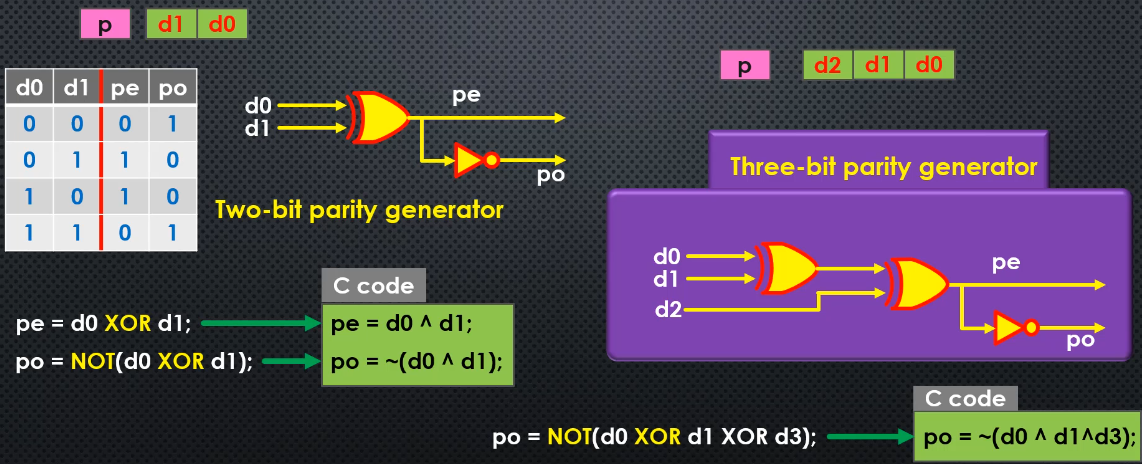
\includegraphics[scale=0.40,frame]{Figures/comb_loop/parity_design}
\caption{Parity bit design for 2 and 3 bit}
\label{fig:comb_loop:parity_design}
\end{figure}

\begin{itemize}

\item The output of the system in the truth table is $p_e$ (for parity even) and $p_o$ (for parity odd)

\end{itemize}

\todo{parity 3 bit desing} \uti{parity 3 bit desing:}

\begin{itemize}

\item \textit{To  derive the truth table for the 3 bit case as in exercice, similar to the 2 bit case}

\item \textit{To do after reviewing the combinational circuit part, and to do it with the VHDL course}

\end{itemize}

Now generalizing the desing concept from 2 or 3 bit to $W$ bit, can be done using a chain of \verb|XOR| gates, as shown in \autoref{fig:comb_loop:parity_w_bit}.

\begin{figure}[h]
\centering
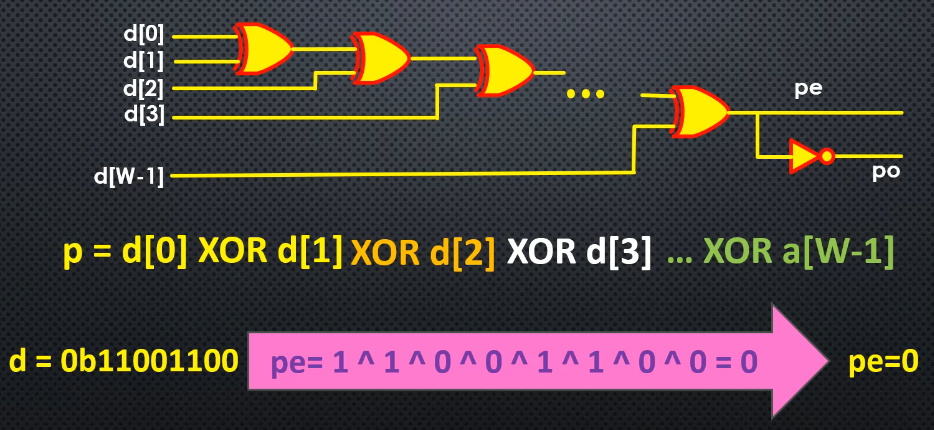
\includegraphics[scale=0.40,frame]{Figures/comb_loop/parity_w_bit}
\caption{Parity bit for $W$ bit data}
\label{fig:comb_loop:parity_w_bit}
\end{figure}

As for the propagation delay $t_p$ for the implementation of \autoref{fig:comb_loop:parity_w_bit}, assuming each \verb|XOR| gate has $\delta$ delay, and we have $(W \, - \, 1)$ \verb|XOR| gate (each 2 data bit line $d[w]$ and $d[\, w + \, 1]$ need 1 \verb|XOR| gate, so for $W$ data bit lines we need $(\, W\, - \, 1\,)$ \verb|XOR| gates ), the total propagation delay is: 

\begin{equation}
t_p \, = \, (W \, - \, 1) \, \delta
\label{eq:tp_parity_bit}
\end{equation}

\subsection{Desing optimization}
\label{sub:design_optim}

\autoref{fig:comb_loop:parity_w_bit} desing can be optimized in terms of $t_p$. Assuming that $W$ is a power of $n$, that is $W \, = \, 2^n$, and due to the assoicativity and commutativity of the \verb|XOR| gates, a balance tree can implement the parity bit generator as shown in \autoref{fig:comb_loop:parity_w_bit_balance_tree}.


\begin{figure}[h]
\centering
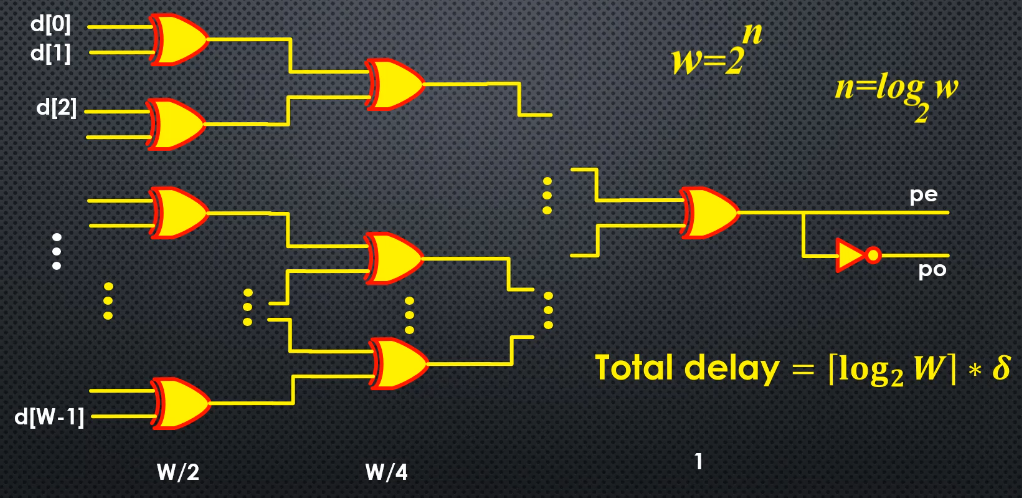
\includegraphics[scale=0.40,frame]{Figures/comb_loop/parity_w_bit_balance_tree}
\caption{Parity bit using balance tree}
\label{fig:comb_loop:parity_w_bit_balance_tree}
\end{figure}

This desing reduce $t_p$ to a function of $\log_2(W)$, which is much smaller than the one in \autoref{eq:tp_parity_bit}.


\begin{equation}
t_p \, = \, \lceil \log_2(W) \rceil \, \times \, \delta
\end{equation}


\newpage
\subsection{Quiz}
\label{sub:quiz_parity_bit}


\underline{Quiz 1:} If we assume $W \, = \, 1024$ bit,

\begin{enumerate}

\item What is number of levels (depth, or layers) of the final balanced tree ?

\item How many \verb|XOR| gates make the final hardware desing ?

\end{enumerate}

\underline{Solution Quiz 1:}

\begin{enumerate}

\item Number of layers equal to $\log_2(1024) \, = \, 10$ levels. 

\item Number of \verb|XOR| gates $1024 \, - \, 1 \, = \, 1023$ 

\end{enumerate}

The final desing for $W \, = \, 1024$ bit is shown in \autoref{fig:comb_loop:quiz_1_parity_bit_param}.

\begin{figure}[h]
\centering
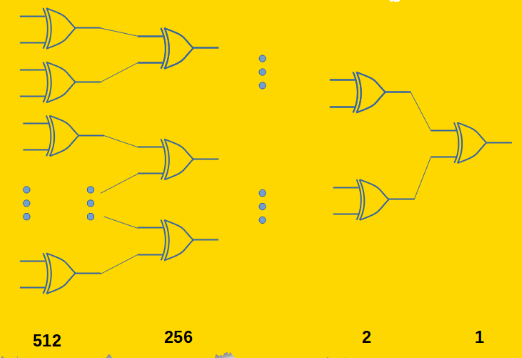
\includegraphics[scale=0.45,frame]{Figures/comb_loop/quiz_1_parity_bit_param}
\caption{Parity bit using balance tree}
\label{fig:comb_loop:quiz_1_parity_bit_param}
\end{figure}


\newpage
\underline{Quiz 2:} Find $t_p$ of an even parity bit generator for an 11 bit data if the delay of an \verb|XOR| gate is 1 ns.\\

\underline{Solution Quiz 2:} \\

\autoref{fig:comb_loop:quiz_11bit_parity} shows the desing using a balanced tree approach for 11 bit data line. 


\begin{figure}[h]
\centering
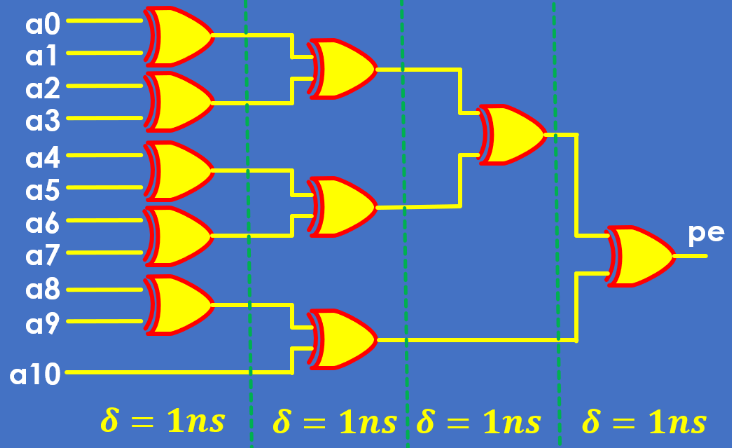
\includegraphics[scale=0.45,frame]{Figures/comb_loop/quiz_11bit_parity}
\caption{Parity bit using balance tree}
\label{fig:comb_loop:quiz_11bit_parity}
\end{figure}

Since the balance tree use a layer approach, each layer has a 1 ns delay even if in 1 layer we have multiple \verb|XOR| gates, where

\begin{itemize}

\item Total number of \verb|XOR| gates $ = \, W \, - \, 1 $

\item Number of \verb|XOR| gates per layer $ = \, \lfloor \displaystyle\frac{W}{2} \rfloor $. 

\end{itemize}

Thus total delay is $t_p \, = \, $ number of layers used $\times$ 1 ns $= \, 4 \, \times \, 1\, = \, 4$ ns.


\newpage
\section{Parity bit in HLS}

Recall from \autoref{sec:parity_bit_design}, that the generalized expression for $W$ bit data lines $d[w]$, take the form of:

\verb|p = d[0] XOR d[1] XOR d[2] ... XOR d[w - 1]|.

The implementation in \verb|HLS| is shown in \autoref{fig:comb_loop:parity_bit_hls}.

\begin{figure}[h]
\centering
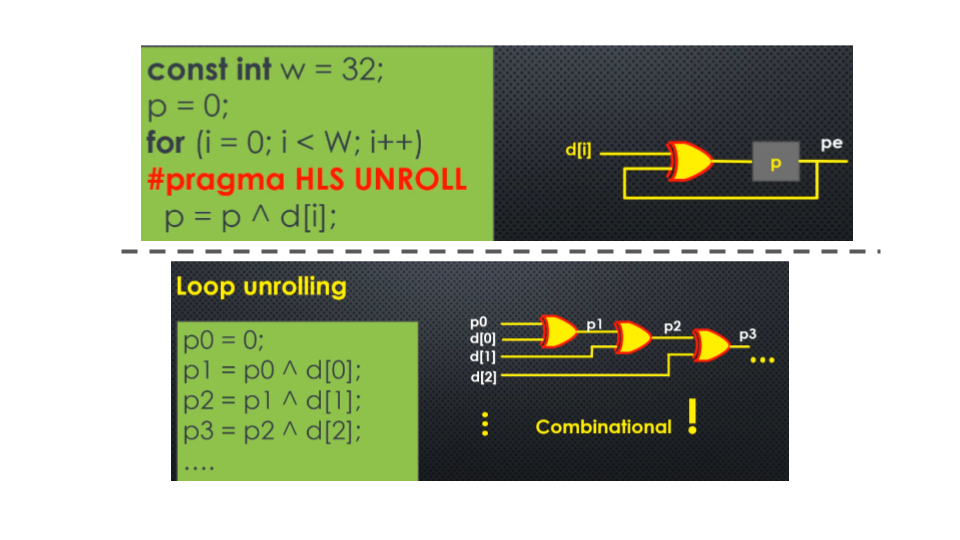
\includegraphics[scale=0.45,frame]{Figures/comb_loop/parity_bit_hls}
\caption{Parity bit HLS implementation}
\label{fig:comb_loop:parity_bit_hls}
\end{figure}

Notice that we use the \verb|#pragma HLS UNROLL| to unroll the \verb|for| loop. By unrolling the \verb|for| loop, we have an equivalent implementation (as shown in the bottom part of \autoref{fig:comb_loop:parity_bit_hls}), where \verb|HLS| tool copy automatically the body of loop statement in each iteration, which result in running the loop statements concurrently and not sequentially.

Whithout the \verb|pragma|, the parity bit by nature needs a result from previous iteration, thus it need some memory to track and save the result, which result in a non-combinational loop.\\

\underline{Note:} In the bottom part of \autoref{fig:comb_loop:parity_bit_hls}, the manually unrolled loop result in a ladder of \verb|XOR| gates, but \verb|HLS| tools handles automatically an optimized impelementation as the balanced tree seen in \ref{sub:design_optim}.


\subsection{Some Work to be done}

\todo{Project Parity-Bit-Vitis} \uti{Project Parity-Bit-Vitis:}

\begin{itemize}

\item \textit{To run the simulation later using Vivado, because in the course it wasn't done}

\item \textit{There is also the usage of the wavefrom viewer, and see for each input we have the correct output}

	\begin{itemize}
	
	\item \textit{I didn't understant this quiet right}	
		
	\item \textit{to be re-done this later}

	\end{itemize}

\end{itemize}

\todo{Waveform viwer in Vitis} \uti{Waveform viwer in Vitis:}

\begin{itemize}

\item \textit{To understand how to use the waveform viwer in Vitis}

\item \textit{How to use with some combinational circuit for example}

\end{itemize}


\newpage
\section{Extra Exercices}

\begin{enumerate}

\item Describe a combinational circuit is HLS to find the even-parity bit of all even bits in an $N$ bit binary data.

\item Describe a combinational circuit in \verb|HLS| to count the number of ones in an $N$ bit binary number. (For example $N\, = \, 345$)

\item Design a combination circuit that returns the even-parity bit of all even bits of a 234-bit input binary number. 

Do not use \verb|for| loop statement. 

\end{enumerate}





\newpage
\section{Summary Combinational Loops}

\begin{itemize}

\item Prallelism and delay:

	\begin{itemize}
	\item A nice demo to illustrate the concept of parallelism and delay is in \ref{eq:tp_parity_bit}
	
	\item The intuition of the exercices is that due to the parallelism properties in FPGA hardware and in the balanced tree desing for parity bit system, $t_p$ is not multiplied, or for example equal to the number of \verb|XOR| gates used in the system
	
	\item \todo{Prallelism and delay} \uti{Prallelism and delay}: 
	
	\textit{To review this concept later, and that I understood this well, when reviewing the logic desing course and VHDL course}
	
	
	\end{itemize}


\end{itemize}









